%Manual for atomistic spin dynamics code
\documentclass{article}

\usepackage{graphicx}
\usepackage{fancyvrb}
\usepackage{amsmath}
\usepackage{mathrsfs}
\usepackage{ulem}
\usepackage[usenames,dvipsnames]{color}
\usepackage{url}
\usepackage[colorlinks=true,linkcolor=blue]{hyperref}
\usepackage{textcomp}

\newcommand\litem[1]{\item{\bfseries #1\enspace}}

\bibliographystyle{unsrt}

\begin{document}
\title{Implementation of the Geodesic Nudged Elastic Band method in UppASD code}
\author{Pavel Bessarab}
\maketitle

\section{Introduction}

Geodesic Nudged Elastic Band (GNEB) method is a method for calculating minimum energy paths (MEPs) for over-the-barrier transitions in magnetic systems. The MEP between two minima is the path in configuration space which lies lowermost on the energy surface. Following an MEP means rotating each magnetic moment in the system in such a way that the energy is minimal with respect to all degrees
of freedom perpendicular to the path. A maximum along an MEP corresponds to a first order saddle point (SP) on the energy surface, and the highest maximum gives an estimate of the activation energy barrier. MEP not only gives the position of SP, but also provides information about microscopic mechanism of the transition, as it represents the path of highest statistical weight.  

The GNEB 
method involves taking an initial guess of a path between the two energy minima,
and systematically bringing that to the nearest MEP. A path is
represented by a discrete chain of states (or 'images') of the system, where the first and the last image are placed at the energy minima corresponding to the stable configurations. In order to distribute the images evenly along the path, springs are introduced between adjacent images. At each image, a local tangent to the path needs to be estimated 
and the force guiding the images towards the nearest MEP is defined 
as the sum of the transverse component of negative energy gradient,
i.e. the true force, and the component of the spring force along the tangent.   
The GNEB force defines the direction of the displacements that bring the
images towards the nearest MEP. The magnitude and exact direction of
the displacement depends on the particular optimization method used in
combination with the GNEB method. A straightforward approach would
be to use the GNEB forces in the Landau-Lifshitz-Gilbert equation instead
of the usual effective fields where the precession term is dropped and then
iterate the equations until convergence to the MEP has been reached. But other optimization schemes can also be used.

Typically, the most important result sought from an GNEB calculation
is the highest energy along the MEP since this gives an estimate of the
activation energy for the transition. The SP will, however, most
likely lie in between GNEB images and the estimate of the maximum energy
then be subject to errors in the interpolation between images. In order to
determine the maximum energy accurately, the highest energy image can be
treated separately during the GNEB optimization. The effective force on this 'climbing image'
(CI) is calculated by zeroing the spring force acting on it and inverting the
parallel component of the true force. In this way, the climbing image is made to move uphill in energy along
the path but downhill in energy perpendicular to the path. The adjacent
images effectively define the appropriate
climbing direction to reach a first order saddle point. After the CI-GNEB
calculation has converged, the position of the climbing image coincides with
the highest SP along the MEP.

An important aspect of the GNEB method is that it is designed so as to account for the curvature of the configuration space arising from the constraint on the length of the magnetic moments, $|\vec{m}_i|=const$. Namely, configuration space of a system consisting of $P$ magnetic moments is a $2P$-dimensional Riemannian manifold, $\mathcal{R}$, corresponding to the direct product of $P$ 2-dimensional spheres~(see Fig.~\ref{fig:1}):
%
\begin{equation}
\label{eq:conf_space}
\mathcal{R} = \prod_{i=1}^P S_i^2,
\end{equation}
%
where $S_i^2$ is a $2$-dimensional unit sphere associated with the $i$-th magnetic moment. The details of the GNEB method are described at length in~\cite{bessarab_2015}.
\begin{figure}[h!]
\centering
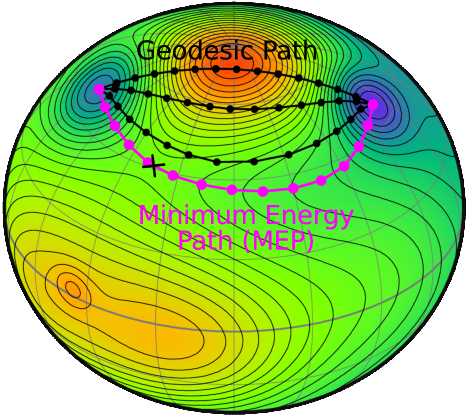
\includegraphics[width=0.7\columnwidth]{fig1.png}
\caption{
A GNEB calculation of an MEP in a single spin system. The positions of the images are shown with filled circles. 
The initial path was chosen to lie 
along the short geodesic path between the energy minima (indicated by blue color) 
and turned out to lie near a maximum (indicated by red color). 
The converged path is shown in pink. 
Two intermediate configurations of the path are also shown. The saddle point is marked with a cross.
$Q=15$ images were used in the calculation. 
}
\label{fig:1}
\end{figure}

Fig.~\ref{fig:1} shows a GNEB calculation of the MEP for a transition of the spin from one minimum to another. 
The initial distribution of images was generated along the short geodesic path connecting the minima. The geodesic path is obviously not an optimal one since it lies close to an energy maximum. 
The images were then iteratively brought to the MEP using the GNEB method with the velocity projection optimization algorithm, as described below.

\section{GNEB calculations in UppASD}

In line with the philosophy of the UppASD package, a standard GNEB calculation involves 3 phases: 
\begin{enumerate}
\item Initialization phase: initial and final configurations are set up.
\item Initial phase (optional): initial and final configurations are relaxed properly to the energy minima.
\item Measurement phase: the MEP between initial and final configurations is found.
\end{enumerate}

The images that give a discrete representation of the path are stored in the ensembles, so when UppASD is used to find MEPs, {\bf Mensemble} is the number of images included in the GNEB calculations. The first ensemble corresponds to the initial state and the last ensemble corresponds to the final state. Therefore, magnetic configuration for the first and for the last ensemble has to be determined. This is done during the initialization phase. Two options are possible: define configurations for the unit cell ({\bf Initmag}=6) or for the whole system ({\bf Initmag}=7). If {\bf Initmag} is set to 6, then two files have to be specified from where the initial and the final configurations are loaded. The structure of the files is identical to that of the {\bf momfile}. If {\bf Initmag} is set to 7, then the initial and the final configurations are loaded from a single file which structure is similar to {\bf moment.$<$simid$>$.out}. The only difference is that the number in the first column in this file corresponds to the ensemble rather than the time step in the {\bf moment.$<$simid$>$.out} file. At least two ensembles must be included in the file: One for the initial configuration and one for the final configuration.

{\bf NOTE:} If {\bf Initmag} is set to 6, the {\bf momfile} has to be provided along with the files for the initial and the final configurations.

{\bf NOTE:} If interaction parameters or the magnitude of magnetic moments have been changed after an UppASD run, where the {\bf do\_prnstruct} had been set to 1, it is recommended to delete the {\bf struct*} files prior to the subsequent UppASD runs so as to have all interaction parameters transferred correctly.

During the initial phase, the initial and the final configurations are relaxed to the energy minima. If the energy minimization has not converged within the predefined number of iterations or the initial and the final states ended up in the same energy minimum, the warning message is displayed. The initial phase can be skipped.

{\bf NOTE:} The GNEB method becomes unstable if the initial and the final states do not correspond to the energy minima. This has to be taken into account when skipping the initial phase.

In the measurement phase, the path between the two relaxed configurations is either generated or loaded from a file and then relaxed to the MEP. GNEB alorithm or CI-GNEB algorithm or both can be used to guide the images towards the MEP. After the path has been converged to the MEP, various properties are extracted based on the calculated MEP, including magnetic configurations along the MEP, energy of the images, interpolated energy along the path, the SP configuration and SP energy as well as effective fields at each image.

{\bf NOTE:} Interpolation of the energy along the path is not only for producing nice figures. Since it is based on both energy and it's derivative (Hermite interpolating polynomials), it can show the indication of an intermediate minimum, which would otherwise not been noticed. If there are intermediate minima along the path, it is recommended to divide the path up into segments and study transitions between each pair of adjacent minima separately.


\section{Input}

In order to perform energy minimization in the initial phase and (CI-)GNEB calculations in the measurement phase, the {\bf ip\_mode} and {\bf mode} parameters need to be set to '{\bf G}'. Other parameters specific for the GNEB calculations which can be defined in {\bf inpsd.dat} file include:

\subsubsection*{amp\_rnd} 
Amplitude of the random noise included in the initial conditions for the initial and final configurations (default: 0.0)

\subsubsection*{amp\_rnd\_path} 
Amplitude of the random noise included in the initial conditions for the path (default: 0.0)

\subsubsection*{do\_gneb} 
Perform GNEB calculations (Y/N, default: Y)

\subsubsection*{do\_gneb\_ci}
Perform CI-GNEB calculations (Y/N, default: N)

{\bf NOTE:} If both {\bf do\_gneb} and {\bf do\_gneb\_ci} are set to 'Y', then a GNEB calculation is performed first. It is therefore advisable to set lower accuracy for the GNEB calculation as compared to that of the CI-GNEB calculation. The accuracy is controlled by {\bf mepftol} and {\bf mepftol\_ci} parameters, see below.

\subsubsection*{do\_norm\_rx}
Normalize reaction coordinate (Y/N, default: N). Reaction coordinate is defined as a displacement along the path connecting the initial and the final states. It can be normalized so that it is equal to zero at the initial state and unity at the final state.

\subsubsection*{initpath}
This entry specifies what initial conditions for the path are used (1 = geodesic path, 2 = load from file, default: 1). Geodesic path is the shortest path between the initial and the final configurations on the $\mathcal{R}$-manifold (see Introduction section). The structure of the file from where the path is loaded is analogous to that of {\bf moment.$<$simid$>$.out}, but the first column corresponds to the image number rather than to the time step. An example of the file from where the transition path including 5 images for two spins can be loaded is shown below:

\begin{Verbatim}
1   1   0.000000   0.000000   1.000000   1.50
1   2   0.000000   0.000000   1.000000   2.21
2   1   0.000000   0.707107   0.707107   1.50
2   2   0.000000  -0.707107   0.707107   2.21
3   1   0.000000   1.000000   0.000000   1.50
3   2   0.000000  -1.000000   0.000000   2.21
4   1   0.000000   0.707107  -0.707107   1.50
4   2   0.000000  -0.707107  -0.707107   2.21
5   1   0.000000   0.000000  -1.000000   1.50
5   2   0.000000   0.000000  -1.000000   2.21
\end{Verbatim}

\subsubsection*{mepftol}
Accuracy of a GNEB calculation (default: 0.001 mRy). If the GNEB force on all of the magnetic vectors in all of the images is smaller than {\bf mepftol}, then the GNEB calculation stops and the path is considered to be converged to the MEP.

\subsubsection*{mepftol\_ci}
Accuracy of a CI-GNEB calculation (default: 0.00001 mRy). If the (CI-)GNEB force on all of the magnetic vectors in all of the images is smaller than {\bf mepftol\_ci}, then the CI-GNEB calculation stops and the path is considered to be converged to the MEP.

\subsubsection*{mepitrmax}
Maximum number of iterations in a (CI-)GNEB calculation (default: 10000000). If the (CI-)GNEB calculation has not converged within {\bf mepitrmax} iterations, the warning message is displayed.

\subsubsection*{meptraj\_step}
Number of iterations between successive writes of intermediate data during a (CI-)GNEB calculation (default: 100). The path is saved to {\bf moment\_path.$<$simid$>$.restart} file. This file can be used to load the path in later simulations ({\bf initpath} = 2). The convergence progress can be monitored using the {\bf force\_mep.txt} file, which includes four columns: iteration number, magnitude of the maximal force, image corresponding to the maximal force and the climbing image number (only appears when a CI-GNEB calculation is performed).

\subsubsection*{minalgo}
Optimization algorithm used for the energy minimization and (CI-)GNEB calculations (1 = velocity projection optimization, default: 1). In the velocity projection optimization (VPO) method, the system is advanced according to equations of motion of a point mass on the $\mathcal{R}$-manifold (see Introduction section). In every iteration, only the component of the velocity parallel to the force is kept, unless it is pointing in a direction opposite to the force, at which point it is zeroed. The advantage of this formulation is that if the force keeps pointing in a similar direction, the system accelerates and approaches the optimal point faster. The VPO algorithm takes two parameters: {\bf vpomass} (mass of the point) and {\bf vpodt} (time step), see below. The VPO method is described in detail in~\cite{bessarab_2015}.

\subsubsection*{minftol}
Accuracy of an energy minimization (default: 1e-9 mRy). If the force on all of the magnetic vectors is smaller than {\bf minftol} then the energy minimization stops and the configuration is considered to be converged to an energy minimum.

\subsubsection*{minitrmax}
Maximum number of iterations in an energy minimization (default: 10000000). If the energy minimization has not converged within {\bf minitrmax} iterations, the warning message is displayed.

\subsubsection*{mintraj\_step}
Number of iterations between successive writes of intermediate data during an energy minimization (default: 100). The initial and the final configurations are saved to {\bf moment\_if.$<$simid$>$.restart} file. This file can be used to load the initial state and the final state in later simulations ({\bf Initmag} = 7). The convergence progress can be monitored using the {\bf force\_min.txt} file, which includes five columns: iteration number, magnitude of the maximal force for the initial configuration, energy of the initial configuration, magnitude of the maximal force for the final configuration, energy of the final configuration.

\subsubsection*{momfile\_f}
Name of the file from where the final configuration is loaded for a unit cell (default: 'momfile\_f'). The structure of the file is identical to that of the {\bf momfile}.

\subsubsection*{momfile\_i}
Name of the file from where the initial configuration is loaded for a unit cell (default: 'momfile\_i'). The structure of the file is identical to that of the {\bf momfile}.

\subsubsection*{restartfile\_if}
Name of the file from where the initial and the final configurations are loaded when the {\bf Initmag} parameter is set to 7 (default: 'nofile').

\subsubsection*{restartfile\_path}
Name of the file from where the path is loaded when the {\bf initpath} parameter is set to 2 (default: 'nofile').

\subsubsection*{sample\_num}
Number of samples in the energy interpolation (default: 500).

\subsubsection*{spring}
Magnitude of the spring constant (default: 0.5).

\subsubsection*{vpodt}
Time step for the VPO algorithm (default: 0.01).

\subsubsection*{vpomass}
Mass of the point in the VPO algorithm (default: 1.0).

\section{Output files}
The following files are created during/after an (CI-)GNEB simulation ({\bf NOTE:} Existing files will be overwritten during the simulation):

\subsubsection*{beff\_$<$im$>$.$<$simid$>$.out}
Prints the effective fields (in mRy) for each image {\bf im}. The format of the file is identical to that of the file containing site-dependent fields. An example of the file for a 5-moment system is shown below:

\begin{Verbatim}
1   2.28492428E-002   2.72329234E-001   1.53792364E-004
2   4.62650976E-002   5.37962272E-001   3.11399574E-004
3   4.85321154E-002   5.37752552E-001   3.26660273E-004
4   5.20003203E-002   5.37412124E-001   3.50007070E-004
5   5.67521235E-002   5.36907167E-001   3.81994383E-004
\end{Verbatim}

\subsubsection*{beff\_sp.$<$simid$>$.out}
Prints the effective fields (in mRy) for the SP configuration.

\subsubsection*{enfit\_path.$<$simid$>$.out}
Prints the interpolated energy along the MEP. Reaction coordinate is stored in the first column, energy is written in the second column, derivative of the energy with respect to the reaction coordinate is written in the third column. Zero of the energy corresponds to the initial state. Number of entries in each column is equal to {\bf sample\_num}.

\subsubsection*{en\_path.$<$simid$>$.out}
Prints the energy of the images. Reaction coordinate is stored in the first column, energy is written in the second column, derivative of the energy with respect to the reaction coordinate is written in the third column. Zero of the energy corresponds to the initial state. Number of entries in each column is equal to {\bf Mensemble}.

\subsubsection*{en\_sp.$<$simid$>$.out}
Prints the reaction coordinate, the energy and derivative of the energy with respect to the reaction coordinate (should be zero) at the SP.

\subsubsection*{force\_mep.txt}
Prints information about the convergence of a (CI-)GNEB calculation. Includes four columns: iteration number, magnitude of the maximal force, image corresponding to the maximal force and the climbing image number (only appears when a CI-GNEB calculation is performed). The file is updated after every {\bf meptraj\_step} iterations.

\subsubsection*{force\_min.txt}
Prints information about the convergence of an energy minimization. Includes five columns: iteration number, magnitude of the maximal force for the initial configuration, energy of the initial configuration, magnitude of the maximal force for the final configuration, energy of the final configuration. The file is updated after every {\bf mintraj\_step} iterations.

\subsubsection*{moment\_if.$<$simid$>$.in}
Prints both the initial and the final magnetic configurations prior to the energy minimization. 

\subsubsection*{moment\_if.$<$simid$>$.out}
Prints both the initial and the final magnetic configurations after the energy minimization. 

\subsubsection*{moment\_if.$<$simid$>$.restart}
Prints both the initial and the final magnetic configurations during the energy minimization. The file is overwritten after every {\bf mintraj\_step} iterations. 

{\bf NOTE:} The structure of {\bf moment\_if.*} files is identical to that described in the {\bf initpath} Subsection, but only two images are included: one for the initial configuration and one for the final configuration. The files can be used to initialize the initial and the final configurations in later simulations ({\bf Initmag} = 7). The files can be used as an input to visualization scripts.

\subsubsection*{moment\_path.$<$simid$>$.in}
Prints the path prior to the (CI-)GNEB optimization. 

\subsubsection*{moment\_path.$<$simid$>$.out}
Prints the path after the (CI-)GNEB optimization. 

\subsubsection*{moment\_path.$<$simid$>$.restart}
Prints the path during the (CI-)GNEB optimization. The file is overwritten after every {\bf meptraj\_step} iterations. 

{\bf NOTE:} The structure of {\bf moment\_path.*} files is identical to that described in the {\bf initpath} Subsection. The files can be used to initialize the path in later simulations ({\bf initpath} = 2). The files can be used as an input to visualization scripts, in which case the advancement of the system along the path will be shown.

\subsubsection*{moment\_sp.$<$simid$>$.out}
Prints the SP configuration. The file can be used as an input to visualization scripts.

\section{Practical advice for a successful (CI-)GNEB calculation}

\subsection{Intermediate minima along the path}
If at an intermediate state of the calculation, an interpolation of the energy ({\bf enfit\_path.$<$simid$>$.out} file) gives an indication of an intermediate minimum, it is recommended to divide the path up into segments and study transitions between each pair of adjacent minima separately. The location of the intermediate minimum should first be carefully identified by carrying out an energy minimization and then start separate GNEB calculations of the MEPs between each pair of adjacent minima. The full MEP is, thereby, obtained as a composition of segments of MEPs, each passing through only one SP.

\subsection{GNEB or CI-GNEB?}
The question arises when to use GNEB and when to use CI-GNEB. The latter is particularly efficient when the energy maximum along the path is well defined. However, there are important examples of magnetic transitions where the barriers are flat, making it hard to identify the highest energy image. Flat barriers appear, for example, when the mechanism of a magnetic transition involves temporary domain wall propagation without significant change in energy~\cite{bessarab_2013}. In such cases, it is better to use the regular GNEB method rather than the CI-GNEB method. A good strategy for finding MEPs is, therefore, to start the calculation using the GNEB method and inspect the energy along the path after a few tens of iterations or when the GNEB forces have dropped below some predefined value (significantly larger than desired accuracy). If there is an indication of a flat barrier, then continue using GNEB until convergence. If the path seems to have a well-defined maximum, then switch to the CI-GNEB method. 

\subsection{Multiple MEPs}
When two or more MEPs connect the same initial and final configurations, the (CI-)GNEB optimization procedure will most likely lead to convergence to the MEP closest to the initial path and some sampling of the various MEPs is needed to find the optimal one, or -- more generally -- all the relevant ones.

\subsection{Number of images}
The number of images included in the (CI-)GNEB calculations should be sufficient to ensure good resolution of the path, but not too large either. Typically, on the order of ten to twenty images are used. When complex paths involving intermediate minima are calculated, it is advisable to divide the path at an intermediate minimum and carry out separate (CI-)GNEB calculation of each segment of the MEP, as discussed above.

\subsection{Random perturbation in the initial conditions}
In some cases, when a highly symmetrical initial path
is used, the (CI-)GNEB can result in a path going through a higher order SP, i.e. a
stationary points on the energy surface which is a maximum with respect to
two or more modes. Therefore, it is advisable to add small
random noise to the initial path to break the symmetries.





\begin{thebibliography}{1}

\bibitem{bessarab_2015} P.F. Bessarab, V.M. Uzdin and H. J\'onsson,
\newblock arXiv:1502.05065

\bibitem{bessarab_2013} P.F. Bessarab, V.M. Uzdin and H. J\'onsson, 
\newblock Phys. Rev. Letters {\bf 110}, 020604 (2013).


\end{thebibliography}

\end{document}
